Gang er en fysisk bevægelse, som benytter involverer hele kroppen til at koordinere bevægelsen. Den følgende beskrivelse af én gangcyklus, tager udgangspunkt i beskrivelsen af bevægelserne for det højre ben. Bevægelserne er dog tilsvarende for det venstre ben. \citep{VaughanDavisOConnor1992,Whittle1990}

En gangcyklus begynder når den højre fod har opnået kontakt med underlaget. Når denne cyklus er påbegyndt, inddeles cyklussen endvidere i to faser; standfasen og svingfasen, hvilket fremgår af \figref{fig:gang_cyklus}. \newline
Standfasen har en varighed svarende til cirka 60\% af en gangcyklus. Dette skyldtes, at standfasen indebærer den tid hvor højre fod er i berøring med jorden. Derimod er svingfasen blot en fase på cirka 30\% af hele gangcyklussen. \citep{VaughanDavisOConnor1992} Svingfasen er den varighed, hvor foden og benet bevæges frem og er derfor ikke i berøring med jorden. Denne fod klargører dermed til den kommende kontakt med jorden, foran den venstre fod som er i berøring med underlaget.

\begin{figure}[H]
	\centering
	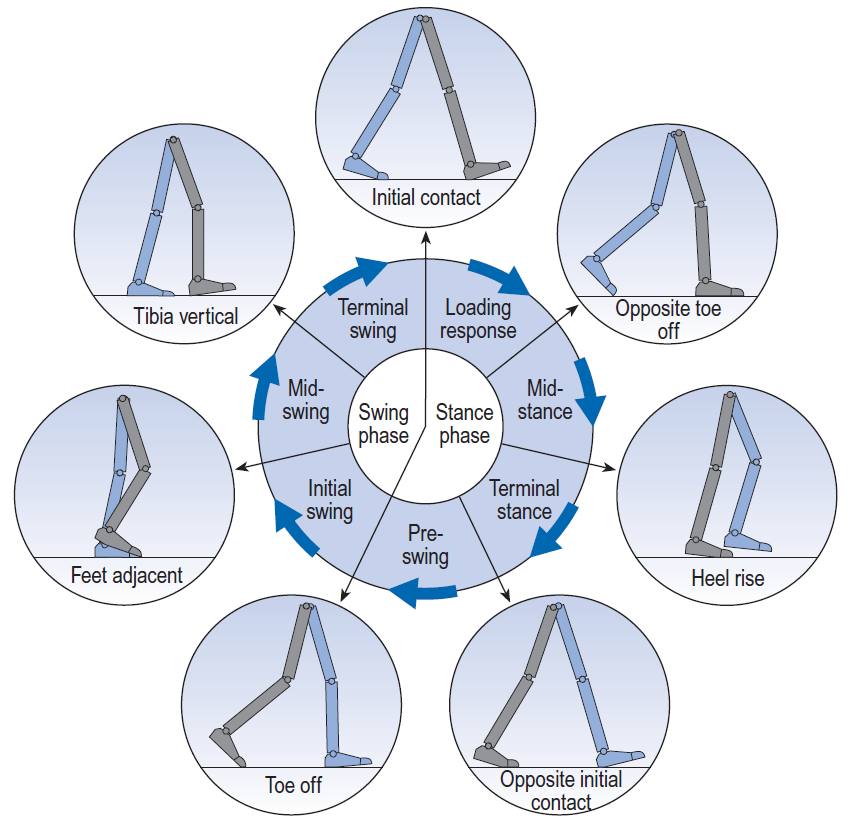
\includegraphics[scale=0.5]{figures/bProblemloesning/gang_cyklus2.png}
	\caption{Figurtekst… \fxnote{SKAL MODIFICERES. Gør så at figuren også har den procentvise fordeling af faserne på} \cite{VaughanDavisOConnor1992}}
	\label{fig:gang_cyklus}
\end{figure}

